\section{Results}\label{sec:results}

I first establish the measure on which the comparison rests, with the decomposition into a Scotland--rUK differential following. I then examine its sensitivity to the measurement choices that, according to \citet{yin2026}, undermine the interpretation of absolute exposure levels. Finally, the differential is translated into the quantities the SFC forecasts.

\subsection{Occupational exposure}\label{sec:saturation}
 
The baseline run scores all 17,945 task--occupation pairs across 894 O*NET occupations. Aggregated to the 104 UK SOC 2020 minor groups on which the regional comparison rests, $E_k$ ranges from 31.7 (building finishing trades) to 84.3 index points (business, research and administrative professionals), with a cross-group standard deviation of 13.6 points. Reassuringly, then, the continuous measure carries the between-occupation variation a compositional comparison needs. The employment-weighted means, 66.7 points in rUK and 65.8 in Scotland, are high by the standards of the survey-based literature, and since the level is the object \cref{sec:method} argues is fragile to the scoring model, I place no weight on them.
 
The classified measure preserves little of this variation. Under the central thresholds, 84 of the 104 minor groups are Complemented, 9 Substituted and 11 Unexposed, so 90.8\% of rUK and 90.9\% of Scottish employment sits above the materiality cut. The classifier is in effect right-censored where once nine-tenths of employment in both regions is coded as exposed, any regional difference in the intensity of exposure is lost and the gap is driven by composition within the small unexposed tail. I therefore treat the continuous index as the primary measure.

\begin{table}[t]
\centering
\caption{Regional exposure indices and the Scotland--rUK differential}
\label{tab:headline}
\small
\begin{tabular}{lcccc}
\toprule
 & Scotland & rUK & Gap & Relative gap \\
\midrule
\multicolumn{5}{l}{\textit{Panel A: continuous indices (index points, 0--100)}} \\
Composite (max operator)   & 65.82 & 66.69 & $-0.86$ & $-1.3\%$ \\
Substitution only          & 38.30 & 38.65 & $-0.35$ & $-0.9\%$ \\
Complementarity            & 62.70 & 63.66 & $-0.96$ & $-1.5\%$ \\
Saturating combination     & 74.74 & 75.51 & $-0.77$ & $-1.0\%$ \\
\addlinespace
\multicolumn{5}{l}{\textit{Panel B: classified employment shares (\%)}} \\
Exposed        & 90.91 & 90.78 & $+0.14$ & $+0.1\%$ \\
Substituted    & 14.90 & 14.21 & $+0.68$ & $+4.8\%$ \\
Complemented   & 76.02 & 76.56 & $-0.55$ & $-0.7\%$ \\
\bottomrule
\end{tabular}
\begin{minipage}{0.92\textwidth}
\vspace{0.4em}\footnotesize
\textit{Notes:} 
Panel A is the continuous exposure index on a 0--100 scale and its gaps are in index points; Panel B reports shares of regional employment and its gaps are in percentage points of employment, under the central thresholds (substitution $\ge 70$, complementarity $\ge 40$).
\end{minipage}
\end{table}
 
\subsection{The Scotland--rUK differential}\label{sec:differential}
 
\cref{tab:headline} contains the headline exposure result. Scotland's employment-weighted continuous exposure is 0.86 index points below rUK on the 0--100 scale (65.82 against 66.69), a relative shortfall of 1.3\%. The sign is stable across exposure operator: the substitution-only index gives $-0.35$ index points, the complementarity index $-0.96$, and the saturating combination $-0.77$. 
%The composed 95\% interval of \cref{sec:interval}, carrying scoring noise and APS sampling error jointly, is $[-1.07, -0.69]$ index points. 
Scotland is therefore less exposed than the rest of the UK, by only a modest margin but with the sign well determined.

%That the interval excludes zero is worth defending rather than asserting, since it states precision within one design and is not an exact coverage statement. As \cref{app:data} records, the person-level bootstrap treats overlapping Labour Force Survey waves as independent draws and ignores the survey's clustering, so it understates the sampling variance of the shares, and it captures sampling variance but not the differential non-response that the 2022--24 fall in LFS response rates makes a live concern. Three things nonetheless keep the sign standing. First, the margin is large relative to any understatement plausible here: the composed standard deviation is 0.101 index points, so zero enters a 95\% interval only if the true standard error is 0.44, a variance inflation of about nineteen. Even if every pooled respondent appeared twice across the four annual files, the effective sample would merely halve and the standard error rise by $\sqrt{2}$; a design effect of nineteen is an order of magnitude beyond what LFS clustering is documented to produce at regional level. Second, non-response enters as a bias in the shares, and closing a gap of 0.86 index points over an observed score range of 32--84 requires moving about 1.6 percentage points of Scottish employment from the least- to the most-exposed minor group, which is the largest genuine share difference anywhere in the 104-group distribution and would have to run entirely one way. Third, the sign does not rest on the interval at all: it holds under all four exposure operators, against the ex-London comparator, in 17 of the 21 SIC sections, under every crosswalk aggregation rule (\cref{tab:crosswalkrules}), and under both alternative scoring models. The caveats of \cref{app:data} bear on the width of the interval, not the direction it lies in.
 
The scale-free form of the result is that Scotland sits about two percentile points below rUK in the UK occupational exposure distribution.
%, a magnitude \cref{sec:crossmodel} shows to be stable across scoring models where the $-0.86$ index-point figure is not, and it is the percentile statement a forecasting body should carry forward. 
%The index-point gap is nonetheless reported throughout, since the decomposition, the propagation and the productivity functional are all defined on that scale, and should be read as the baseline model's expression of a finding whose robust content is ordinal.
The differential is small because the two regional labour markets are similar. Their employment-share vectors are close to collinear, with the largest difference across the 104 minor groups (functional managers and directors) amounting to only 1.6 percentage points of employment.
%and \cref{app:descriptives} expands on the underlying composition alongside the wider structural differences between the two economies. 
Over the observed score range of 32--84 index points, no assignment of exposure can produce a large aggregate gap from compositional differences so small. 
%The continuous index adds the ability to recover the sign of that gap and trace it to its underlying components.
 
%The aggregation to minor groups masks any Scotland--rUK employment sorting within occupations, and the APS data, which resolves employment only to the minor group, cannot verify whether such sorting exists. Yet the between-group pattern of \cref{tab:decomposition} suggests it does: Scotland is underweight in the higher-exposure variants of the same broad occupations. If true, the measured differential is conservative. As for the fiscal implications, even a doubled gap translates into a productivity differential of the same order, leaving \cref{sec:productivity} intact.
 
\subsection{Anatomy of the differential}\label{sec:anatomy}

\cref{tab:decomposition} reports the largest per-occupation contributions $\Delta\eta_k (E_k - \Ebar_{\rUK})$ on each side, with the anatomy visualised into coarser groups in \cref{fig:comp}. An occupation's contribution is the product of two signs: whether Scotland is over- or under-represented in occupation $k$, and whether that occupation sits above or below the rUK average exposure $\Ebar_{\rUK}$ of 66.7. A contribution is negative either when Scotland is underweight in above-average work or when it is overweight in below-average work, and vice versa for positive cases.

Scotland is underweight in highly exposed professional occupations (functional managers and directors alone contribute $-0.17$ points and IT professionals $-0.11$) along with being overweight in service occupations that sit below the average, notably caring personal services ($-0.17$) and other elementary services ($-0.16$). 

The offsetting positive contributions arise from Scotland being underweight in some low-exposure work, chiefly childcare and related personal services ($+0.09$) and construction and building trades ($+0.06$), whilst being overweight in a few high-exposure occupations, among them engineering professionals ($+0.05$), government administration ($+0.05$) and customer service ($+0.04$). The differential emerges from many small and economically coherent compositional differences rather than from a few influential occupations.

 
\begin{table}[t]
\centering
\caption{Decomposition of the continuous differential: largest contributions}
\label{tab:decomposition}
\small
\begin{tabular}{clccc}
\toprule
SOC & Minor group & $E_k$ & $\Delta\eta_k$ (pp) & Contribution (pp) \\
\midrule
113 & Functional managers and directors        & 77.5 & $-1.58$ & $-0.171$ \\
613 & Caring personal services                 & 51.2 & $+1.07$ & $-0.165$ \\
926 & Other elementary services                & 46.3 & $+0.76$ & $-0.155$ \\
922 & Elementary cleaning                      & 39.1 & $+0.51$ & $-0.140$ \\
213 & IT professionals                         & 80.9 & $-0.79$ & $-0.112$ \\
\\
611 & Childcare and related personal services  & 47.5 & $-0.49$ & $+0.094$ \\
531 & Construction and building trades         & 37.4 & $-0.20$ & $+0.059$ \\
212 & Engineering professionals                & 79.3 & $+0.42$ & $+0.053$ \\
411 & Administrative: government and related   & 79.4 & $+0.39$ & $+0.050$ \\
721 & Customer service occupations             & 79.4 & $+0.35$ & $+0.044$ \\
\bottomrule
\end{tabular}
\begin{minipage}{0.92\textwidth}
\vspace{0.4em}\footnotesize
\textit{Notes:} Contributions are $\Delta\eta_k (E_k - \Ebar_{\rUK})$, in index points, summing exactly to the composite gap of $-0.86$ index points; the five largest on each side are shown. $E_k$ is on the 0--100 exposure scale and $\Delta\eta_k$ is the Scotland-minus-rUK difference in the within-region employment share, in percentage points of employment.
\end{minipage}
\end{table}

\begin{figure}
    \centering
    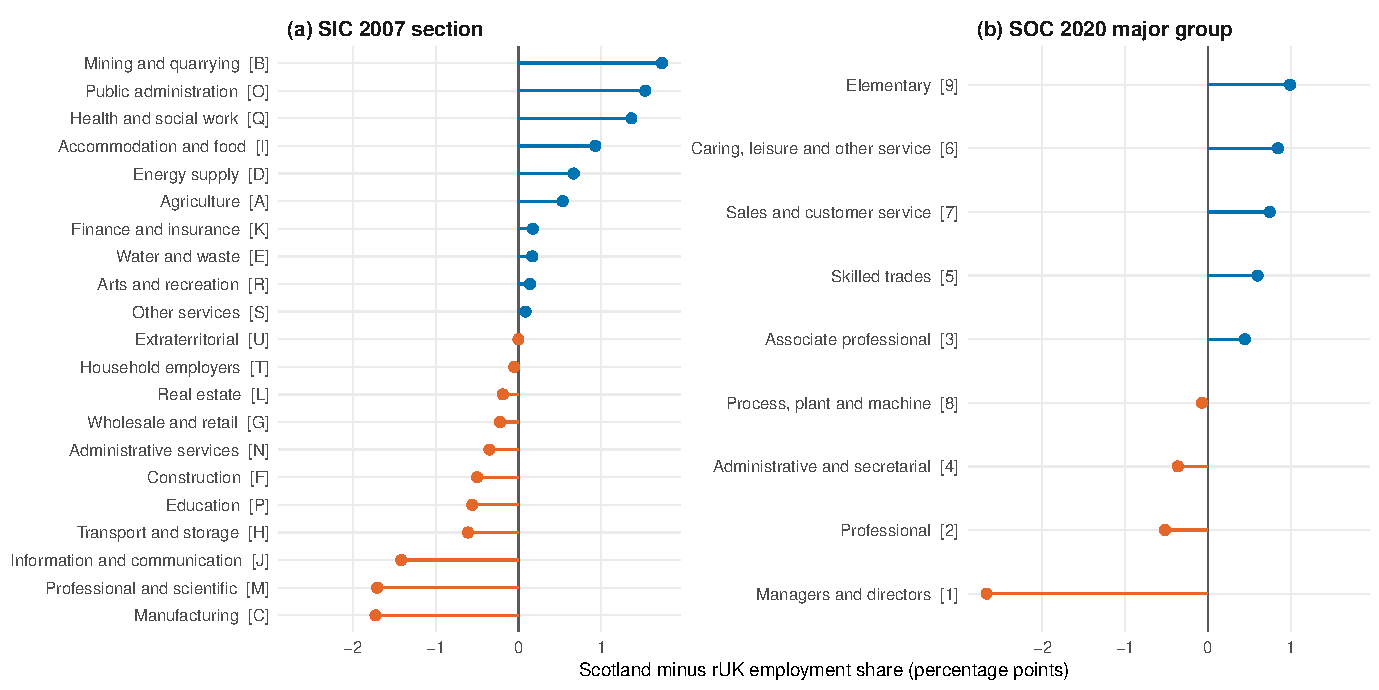
\includegraphics[width=1.0\linewidth]{figures/fig1_composition.pdf}
    \caption{Orange indicates relative employment shortfall, with blue relative excess.}
    \label{fig:comp}
\end{figure}

%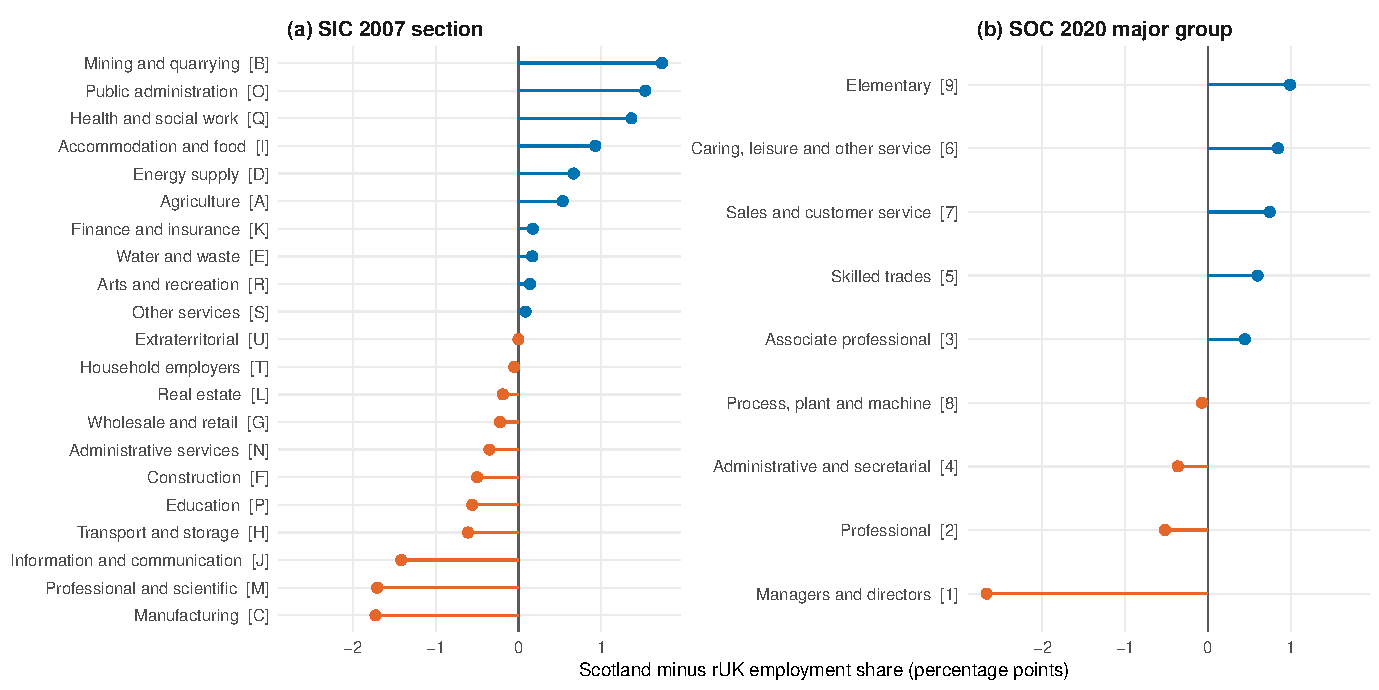
\includepdf[pages=1, scale=0.8, pagecommand={}]{figures/fig1_composition.pdf}
 
Nor is the differential solely a London effect. London's index is 69.30, compared with 66.33 for the UK excluding London, and thus Scotland's 65.82 remains 0.51 index points below the ex-London comparator. That is, excluding London closes 41\% of the headline gap, but it does not eliminate it. The professional-management underweight persists (functional managers still contribute $-0.14$ points) as does the relative concentration in the care-sector. Scotland ranks fifth among the twelve UK nations and regions, behind London, the South East, the East of England, and the North West. The appropriate conclusion is not that Scotland is unusually insulated from AI exposure, but rather that London is unusually exposed, with Scotland sitting slightly below the middle of a distribution that spans barely 2.5 index points once London is excluded.

Expressed as a regression within one-digit occupational major groups, the same pattern holds on both the log-employment and employment-share margins (\cref{app:specifications}), so the gap is not solely a matter of Scotland carrying fewer of the broad occupational families in which exposed work concentrates. 
%The first-difference specification is uninformative, and I read it as such rather than as evidence of no differential response.\footnote{The first-difference interaction is $-0.077$ (SE 0.078). Three annual transitions over 104 minor groups, with 23 of the pooled Scottish groups containing fewer than 100 respondents across the four waves, cannot identify a dynamic effect of this size; the employment weights contain the damage but cannot repair it.}
 
%The industry decomposition points the same way. Roughly three-quarters to four-fifths of the differential arises within industries rather than through Scotland's sectoral structure (\cref{tab:industry}), with the within-industry term is negative in 17 of the 21 SIC sections (\cref{tab:industrysections}). The industry-mix term is small because sectoral differences net out: Scotland is underweight in professional, scientific and information services but overweight in public administration, mining and energy, and only marginally different in finance, so the gap is a professional-services phenomenon rather than a financial one.
%The industry section-by-section breakdown in \cref{tab:industrysections} shows that the within-industry gap is pervasive rather than concentrated. That is, Scottish employment sits lower on the exposure gradient in every large section, with health and social work, wholesale and retail, and professional and technical activities carrying the largest within-industry contributions by virtue of their employment weight. The exception is education, where Scottish employment sits slightly higher on the gradient; the sections with the most extreme within-industry exposure gaps are instead tiny ones, such as extraterritorial bodies and household employers, whose negligible employment share leaves them immaterial to the total.
 
%\begin{table}[t]
%\centering
%\caption{Industry-mix and within-industry components of the differential}
%\label{tab:industry}
%\small
%% Auto-generated by the analysis pipeline -- do not edit by hand.
% \input{} inside a table environment; requires \usepackage{booktabs}.
\begin{tabular}{l r r}
\toprule
Term & Ordering A (rUK exposure, Scottish shares) & Ordering B (Scottish exposure, rUK shares) \\
\midrule
Industry mix & -0.2094 & -0.1708 \\
Within industry & -0.6561 & -0.6947 \\
Total (= gap) & -0.8655 & -0.8655 \\
\bottomrule
\end{tabular}

%\begin{minipage}{0.92\textwidth}
%\vspace{0.4em}\footnotesize
%\textit{Notes:} Index points on the 0--100 exposure scale. Employment is split by SIC 2007 section on the pooled APS 2022--2025 sample for which industry is recorded and the occupation matches a scored minor group, so the total differs slightly from the headline gap of \cref{tab:headline}. Per-section contributions are in \cref{tab:industrysections}.
%\end{minipage}
%\end{table}
 
%\subsection{Substitution against complementarity}\label{sec:channels}
 
%The channel through which Scotland is exposed also differs from rUK, and the distinction matters because substitution and complementarity carry opposite-signed productivity implications in the projection of \cref{sec:productivity}. Panel B of \cref{tab:headline} shows Scotland's classified substituted employment share 0.68 percentage points above rUK (14.90\% against 14.21\%), even though its continuous substitution intensity is 0.35 points lower. Scotland is overweight in occupations where the substitution score exceeds the complementarity score, such as sales assistants and customer-service occupations, whilst underweight in the administrative minor groups with the highest substitution intensities. The precise magnitude depends on how exposure is classified, but the qualitative pattern is stable across specifications. That is, Scottish exposure is relatively more concentrated in substitution-dominated occupations, even though both continuous channel indices are lower than in rUK. The continuous indices make the same point without the classifier: Scotland's substitution deficit is proportionally smaller than its complementarity deficit ($-0.9\%$ against $-1.5\%$), so its exposure leans towards substitution in relative terms even while sitting below rUK on both channels. For that reason, the productivity projection in \cref{sec:productivity} treats the two channels separately throughout.
 
\subsection{Scoring noise, sensitivity, and the composed interval}\label{sec:interval}
 
The calibration experiment delivers the within-model noise parameters. Across the meaning-preserving variants (V1--V3 of \cref{tab:calibration}), the standard deviation of an occupation's total score ranges from 1.3 to 2.4 index points across the five occupational families, with task-level standard deviations of 3.4--5.1 index points for substitution and 3.6--6.0 for complementarity. Now, the estimand variants shift levels by much more. Shortening the horizon to five years (V4) moves composites by $-1.5$ index points on average, and collapsing the two-dimensional rubric to a single score (V5) moves them by $-11.6$. Interestingly, the cross-occupation correlations with the V0 baseline remain 0.998 and 0.956, so changing the question moves every level but barely moves the ordering of occupations. That is the same common-mode structure \cref{prop:cancellation} formalises, with levels highly specification-dependent and relative positions not. 
%That is why I place little weight on the levels of \cref{sec:saturation} and focus instead on the differential.\footnote{The near-invariance to the horizon is a construct caveat rather than a reassurance: the model appears to rate what a task is amenable to more than what is achievable within the stated window. Any component of that insensitivity common across occupations is innocuous for the differential by \cref{prop:cancellation}, but it bears on the projection of \cref{sec:productivity}, where the ten-year horizon does economic work, and I return to it there.}
 
\begin{table}[t]
\centering
\caption{Propagated uncertainty in the differential $\protect\dEbar$}
\label{tab:propagation}
\small
\begin{tabular}{lccccc}
\toprule
Component & $\rho$ & Mean & SD & 2.5\% & 97.5\% \\
\midrule
Scoring only  & 0   & $-0.863$ & 0.017 & $-0.897$ & $-0.830$ \\
Scoring only  & 0.2 & $-0.864$ & 0.031 & $-0.922$ & $-0.801$ \\
Scoring only  & 0.4 & $-0.864$ & 0.039 & $-0.938$ & $-0.788$ \\
Sampling only & --  & $-0.864$ & 0.099 & $-1.070$ & $-0.690$ \\
Composed      & 0   & $-0.863$ & 0.101 & $-1.069$ & $-0.688$ \\
Composed      & 0.2 & $-0.862$ & 0.103 & $-1.086$ & $-0.677$ \\
Composed      & 0.4 & $-0.865$ & 0.108 & $-1.091$ & $-0.675$ \\
\bottomrule
\end{tabular}
\begin{minipage}{0.92\textwidth}
\vspace{0.4em}\footnotesize
\textit{Notes:} Index points on the 0--100 exposure scale; 1,000 draws per row. Scoring draws perturb occupation composites with the calibrated $\sigma_g$, correlated within occupational family at $\rho$; sampling draws bootstrap the employment shares over persons within region and year.
\end{minipage}
\end{table}
 
\cref{tab:propagation} propagates the noise, with each draw perturbing the occupation scores once and feeding both regions the same perturbed vector, such that scoring noise is common-mode across regions by construction, and its near-total cancellation in the differential. Thus, the scoring rows are a numerical illustration of \cref{prop:cancellation} and do not quantify uncertainty in the gap. The relevant uncertainty comes from sampling. Bootstrapping the employment shares widens the SD to 0.099 index points, and the composed interval at the most conservative within-family correlation is $[-1.09, -0.68]$ index points, with all 1,000 composed draws negative. Together this frames the headline exposure result as $\dEbar = -0.86$ index points, with 95\% interval $[-1.07, -0.69]$, most of whose width comes from survey sampling. 
%Because the chain from the index to the net position is a linear functional with region-common coefficients (\cref{cor:functionals}), these rows are also the measurement rows of the fiscal error in \cref{sec:fiscal}, rescaled but not recomputed.

%\subsection{Fragility of the classified gap, robustness of the continuous gap}\label{sec:fragility}
 
%The classified gap changes sign under reasonable variations in its own construction whereas the continuous gap does not. At the central thresholds Scotland's exposed share exceeds rUK's by 0.14 percentage points, at the low thresholds by 0.19 points, and at the high thresholds the sign reverses to $-1.36$ points. A measure whose sign depends on the threshold pair is a diagnostic of its own construction, and the mechanism is the censoring of \cref{sec:saturation}: with 91\% of employment above the cut, the classified gap is generated by a handful of share differences in the unexposed tail, and moving the cut relocates the tail. The continuous gap, by contrast, is negative under all four operators, under both classification schemes' underlying scores, and at every point of the uncertainty analysis below.
 
%Classification stability behaves consistently with this reading. Across the meaning-preserving variants, 55.0\% of the near-boundary calibration occupations flip class against 6.0\% of the randomly drawn ones, so instability concentrates where it should. It does not propagate: no occupation and no minor group falls below the stability landmark of \cref{app:calibration}, so the flag never binds, and excluding minor groups by average stability leaves the classified gap unchanged to the fourth decimal place at every cutoff up to 0.85. The flipping occupations carry small and regionally similar employment shares.

\subsection{Cross-model stability of the differential}\label{sec:crossmodel}
 
As \citet{yin2026} show, choice of language model introduces a source of error that averaging cannot remove and therefore provides a direct test of \cref{prop:cancellation}. I re-scored all task--occupation pairs on two additional models, GPT-4o (a different provider) and Claude Haiku 4.5 (a lower tier of the same provider), and recomputed the differential from each.
 
\begin{table}[t]
\centering
\caption{Cross-model stability of the differential}
\label{tab:crossmodel}
\small
\begin{tabular}{llccc}
\toprule
Scoring model & Contrast & Mean bias & $\dEbar$ &
$\operatorname{corr}(b^{M}_k, \Delta\eta_k)$ \\
\midrule
Claude Sonnet 4.6 & baseline                   & --- & $-0.86$ & --- \\
Claude Haiku 4.5  & same provider, lower tier  & 3.5 & $-0.53$ & $-0.24$ \\
GPT-4o            & different provider         & 9.1 & $-0.43$ & $-0.23$ \\
\bottomrule
\end{tabular}
\begin{minipage}{0.92\textwidth}
\vspace{0.4em}\footnotesize
\textit{Notes:} Index points of the 0--100 scale. ``Mean bias'' is the mean absolute occupation-level score difference from the Sonnet baseline; $\dEbar$ is the Scotland--rUK differential recomputed from each model's scores; $b^{M}_k$ is the minor-group score difference from baseline, in index points, and $\Delta\eta_k$ the Scotland--rUK employment-share gap, and so the final column is the empirical surviving term in \cref{eq:prop1}.
\end{minipage}
\end{table}
 
The levels behave as predicted, with the alternative models disagreeing with the Sonnet baseline about absolute exposure by a mean occupation-level bias of 3.5 index points for Haiku and 9.1 for GPT-4o, with the latter divergence being of the order Yin et al. documents across frontier models. As anticipated, the differential, however, moves far less. Against a baseline gap of $-0.86$ index points, Haiku returns $-0.53$ and GPT-4o $-0.43$, so the differencing removes much, but not all, of the model disagreement. That much is \cref{prop:cancellation} doing its work on the additive component of the bias.

By \Cref{cor:affine}, we can say the cross-model differences are systematic rather than idiosyncratic. In both alternative models the bias is strongly correlated with the exposure level itself (0.88 for Haiku, 0.95 for GPT-4o), implying a compression of the scale rather than a simple shift.\footnote{This is a non-classical, mean-reverting error of the kind validation studies of survey data routinely find \citep{bound1991}, with the difference that here there is no absolute truth to revert towards, only a baseline that is itself a model.} The employment-weighted standard deviation of the minor-group scores falls from 13.58 index points under Sonnet to 9.59 under Haiku and 7.55 under GPT-4o, implying affine slopes of $c^{M} = 0.71$ and $0.56$. \Cref{eq:cor2} then predicts differentials of $-0.61$ and $-0.48$ from compression alone, against realised values of $-0.53$ and $-0.43$, so the affine term accounts for roughly three-quarters of the movement in the Haiku gap and nine-tenths in the GPT-4o gap. Compression pulls the highest-exposure occupations down and Scotland is underweight in exactly those, ultimately reading as a 'smaller' differential.
%, which is how a multiplicative disagreement that \cref{eq:decomposition} cannot represent presents itself in \cref{eq:prop1}.
 
Parts (ii) and (iii) of \cref{cor:affine} tell us that dividing by each model's score dispersion removes any affine rescaling and percentile ranks remove any monotone one. Under these transformations the raw gaps of $-0.86$, $-0.53$, and $-0.43$ index points become $-0.064$, $-0.055$, and $-0.057$ standard-deviation units and $-1.97$, $-1.76$ and $-2.01$ percentile points (\cref{tab:crossmodelstd}). The two-fold disagreement in index points collapses to about 13\%, and GPT-4o, whose raw gap lies outside the within-model interval of \cref{tab:propagation}, lands within 2\% of the baseline in percentile terms. These standardised gaps measure how much of the disagreement concerns Scotland's position within the distribution, and on that the three models are close.
%\footnote{\Cref{cor:crossmodel} bounds that residual: the cross-model movement cannot exceed $\tfrac{1}{100}\lVert\Delta\eta\rVert\,\lVert b^{M} - \bar{b}^{M}\rVert$, which is 1.36 index points for Haiku and 1.88 for GPT-4o, so the realised displacements of $-0.33$ and $-0.43$ sit at under a quarter of the worst case.}
 
\begin{table}[t]
\centering
\caption{Scale-free cross-model differentials}
\label{tab:crossmodelstd}
\small
\begin{tabular}{l r r r r}
\toprule
Model & Score SD & Raw gap & SD-unit gap & Percentile gap \\
 & (index pts) & (index pts) & (SDs) & (pctile pts) \\
\midrule
Claude Sonnet 4.6 (baseline) & 13.582 & -0.863 & -0.0636 & -1.966 \\
Claude Haiku 4.5 & 9.593 & -0.531 & -0.0554 & -1.756 \\
GPT-4o (2024-11-20) & 7.549 & -0.431 & -0.0571 & -2.008 \\
\bottomrule
\end{tabular}

\begin{minipage}{0.92\textwidth}
\vspace{0.4em}\footnotesize
\textit{Notes:} The score SD is the UK-employment-weighted standard deviation of the 104 minor-group scores under each model. The SD-unit gap divides the index-point gap by that dispersion, removing any affine rescaling; the percentile gap replaces each score with its UK-employment-weighted percentile rank, removing any monotone rescaling. 
\end{minipage}
\end{table}
 
%This narrows the claim and improves its foundation. 
The sign, the compositional structure, and the scale-free magnitude of about two percentile points all survive a change of scoring model, with \cref{cor:affine} guaranteeing the last against any monotone rescaling. Conversely, the index-point does not survive, ranging from $-0.43$ to $-0.86$ because the models disagree about the dispersion of the index far more than about Scotland's position within it. I therefore report the scale-free magnitude as the headline, with $-0.86$ index points as the baseline model's expression of it. 
%This is also the largest single source of uncertainty in the fiscal figure of \cref{sec:fiscal}, and \cref{sec:budget} sets it against the others.

\subsection{Wage gradients: propagation at the worker level}\label{sec:wages}

The wage regression one, serves as the micro counterpart of the aggregate propagation, and two, supplies the exposure--pay alignment so the estimated Scottish gradient is an input to the fiscal translation rather than a free-standing result.

\begin{table}[t]
\centering
\caption{Exposure--wage regression}
\label{tab:wagespecs}
\begin{threeparttable}
\small
\setlength{\tabcolsep}{5pt}
\renewcommand{\arraystretch}{1.05}
\begin{tabular}{l cccc}
\toprule
 & (1) & (2) & (3) & (4) \\
 & Baseline & $+$Controls & $+$Region & $+$London \\
 & (full) &  & FE & slope \\
\midrule
Exposure $E$ & $1.276^{***}$ & $0.941^{***}$ & $0.913^{***}$ & $0.884^{***}$ \\
 & $(0.170)$ & $(0.144)$ & $(0.143)$ & $(0.143)$ \\
\addlinespace[2pt]
Exposure $\times$ Scotland & $-0.300^{***}$ & $-0.269^{***}$ & $-0.216^{***}$ & $-0.187^{***}$ \\
 & $(0.065)$ & $(0.062)$ & $(0.056)$ & $(0.058)$ \\
\addlinespace[2pt]
Scotland & $0.204^{***}$ & $0.173^{***}$ &  & $0.138^{***}$ \\
 & $(0.044)$ & $(0.042)$ &  & $(0.040)$ \\
\addlinespace[2pt]
Exposure $\times$ London &  &  &  & $0.354^{***}$ \\
 &  &  &  & $(0.059)$ \\
\addlinespace[2pt]
London &  &  &  & $-0.118^{***}$ \\
 &  &  &  & $(0.039)$ \\
\addlinespace[2pt]
\midrule
Demographic controls\tnote{a} & Yes & Yes & Yes & Yes \\
Added controls\tnote{b} &  & Yes & Yes & Yes \\
Industry FE & Yes & Yes & Yes & Yes \\
Year FE & Yes & Yes & Yes & Yes \\
Region (GOR) FE &  &  & Yes &  \\
Clustering & Occ. & Occ. & Occ. & Occ. \\
Sample & Full & GOR & GOR & GOR \\
\addlinespace[2pt]
Observations & 176,444 & 176,024 & 176,024 & 176,024 \\
Within $R^2$ & 0.174 & 0.235 & 0.226 & 0.243 \\
\bottomrule
\end{tabular}
\begin{tablenotes}[flushleft]
\footnotesize
\item Dependent variable: log gross hourly pay. Worker-level regressions
of \cref{eq:wage} on the pooled APS 2022--2025, weighted by the APS income
weight. Standard errors, clustered by occupation (the level at which the
exposure score varies), in parentheses. Column (1) is the full-sample
baseline; columns (2)--(4) add the controls of note b and restrict to
observations with an observed regional code, so column (2) is the
like-for-like comparator for the London treatments in (3)--(4). The
Scotland main effect is absorbed by the regional fixed effects in column
(3) and is therefore not separately estimable.
\item[a] Age, age$^2$, sex, and full-time/part-time status.
\item[b] Highest qualification (education) and a public-sector indicator.
\item[] $^{*}\,p<0.1$, $^{**}\,p<0.05$, $^{***}\,p<0.01$.
\end{tablenotes}
\end{threeparttable}

\end{table}

Higher-exposure occupations pay markedly more, reflecting how exposure aligns with professional and cognitive task content. The coefficient is 1.276 (SE 0.170), so each ten index points of exposure carries about 13.6\% higher pay, implying that pay differs by 95.6\% across the observed range of 31.7 to 84.3 index points. The Scotland interaction of $-0.300$ implies that the Scottish gradient is 0.976 against 1.276 in the rUK, close to a quarter flatter, indicating ten index points of exposure carry about 10.3\% higher pay in Scotland, 3.3\% lower than rUK.
%\footnote{Clustering by occupation $\times$ region gives a standard error of 0.226 on the same point estimate. That choice treats the identical score on the two sides of the border as two independent regressors and assumes away the cross-region error covariance within an occupation, which the interaction contrast nets out; occupation clusters nest occupation $\times$ region clusters and are the appropriate level.} 
Within-occupation wages therefore rise less steeply with exposure in Scotland than in the rUK.

Adding highest qualification and a public-sector indicator (\cref{tab:wagespecs}, column 2) cuts the exposure gradient from 1.276 to 0.941 but barely moves the Scotland interaction, so the flatter Scottish gradient is not a proxy for its qualification mix or its larger public sector. Giving London its own level and its own exposure slope (column 4) removes about three-tenths of the controlled interaction, so roughly a third of it is the capital and the remainder belongs to Scotland. 
Against the ex-London comparator the Scottish return to exposure is roughly a fifth lower than in the rest of the UK (0.697 against 0.884), paying roughly 8\% more in the least exposed occupations, drawing level at 73.8 index points, and about 2\% less at the most exposed end. Scotland has less exposed employment and pays less for the exposed work it has, both of which compound in the fiscal translation of \cref{sec:fiscal}.

The wage regression carries a variable with error because the exposure scores are estimates, and random error in a regressor pulls its coefficient towards zero. How much depends on the noise relative to the real variation in exposure across occupations, and here scores run from 31.7 to 84.3 while the uncertainty about any one of them is a small fraction of that ($\lambda = 0.016$). The correction is accordingly 1.6\%: the gradient moves from 1.276 to 1.297 and the Scotland interaction from $-0.300$ to $-0.305$, and \cref{app:additional} shows even that to be an upper bound. Scoring noise is immaterial here, as \cref{tab:propagation} finds it to be in the aggregate, with the largest uncertainty component from survey sampling. 

%The flat pass-through of \cref{sec:fiscal} spreads the earnings differential evenly across workers, whereas the mechanism of \cref{eq:tfp} concentrates it on exposed occupations, and \cref{app:elasticity} prices that difference with an incidence-weighted elasticity $\varepsilon^{E}$. What that correction needs is the alignment between exposure and pay, which is what $\beta_1$ measures: exposed work sits higher in the earnings distribution and so at higher marginal rates, and that is the whole reason $\varepsilon^{E}$ exceeds $\varepsilon$. The Scotland interaction says how much of the alignment survives north of the border, and the answer is about four-fifths of it. That is why the correction computed on Scottish data is small, at $\varepsilon^{E} = 1.974$ against $\varepsilon = 1.922$: a flatter Scottish exposure--pay schedule leaves less for the incidence weighting to recover, so the flat elasticity carried through \cref{tab:fiscal} understates the revenue consequence by 2.7\% and the reported figure is conservative on this margin. The gradient is therefore less a third demonstration of propagation than the empirical content behind one of the four multiplicative steps of \cref{sec:fiscal}.

One caveat on the wage exercises arises since gross hourly pay is recorded on the APS for employees only. Therefore, the estimates describe the employee earnings distribution but exclude the self-employed, who are disproportionately concentrated in the professional occupations sitting at the top of the exposure distribution.